\section{Séance 9}

\paragraph{1. } Donnez une autre représentation planaire du graphe suivant où la face spécifiée devient la face extérieure. 

\begin{center}
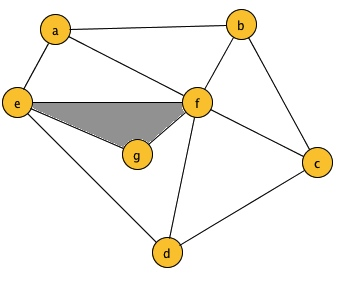
\includegraphics[scale=.4]{ape9_ex1_1.jpg} 
\end{center}

\textit{Solution}

\begin{center}
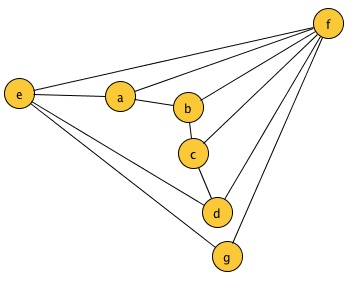
\includegraphics[scale=.4]{ape9_ex1_2.jpg} 
\end{center}

\paragraph{2. }Un graphe planaire peut-il être représenté sur un cylindre bi-infini sans que ses arêtes ne se croisent? La réciproque est-elle vraie? Et pour un graphe sur un tore? 

\paragraph{3. }Les graphes suivants sont-ils planaires?

\begin{tabular}{lcccr}
a)
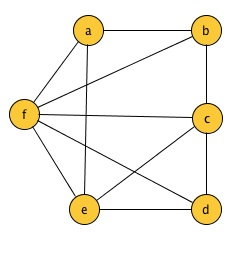
\includegraphics[scale=.4]{ape9_ex3_a_1.jpg}
& $\qquad$ & b) 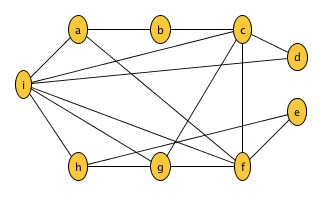
\includegraphics[scale=.4]{ape9_ex3_b_1.jpg}
& $\qquad$ & c) 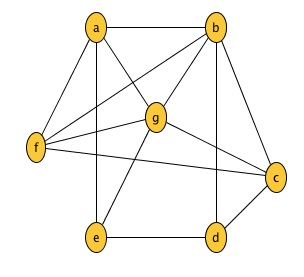
\includegraphics[scale=.4]{ape9_ex3_c_1.jpg} \\
\end{tabular} 

\bigskip 


\textit{Solution}

\begin{tabular}{lcr}
a) Oui
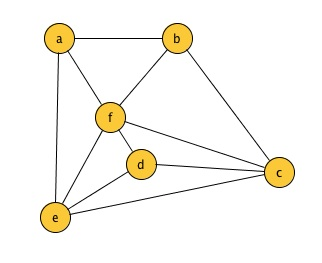
\includegraphics[scale=.4]{ape9_ex3_a_2.jpg}
& $\qquad$ & b) Oui 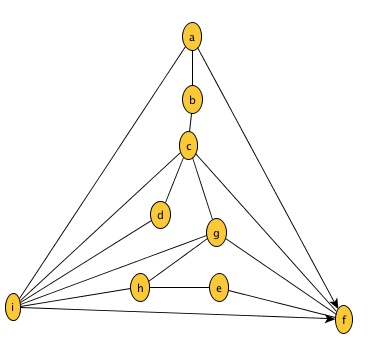
\includegraphics[scale=.4]{ape9_ex3_b_2.jpg}
\end{tabular}

\paragraph{4. }Supposez qu'un graphe connexe planaire a 6 sommets, chacun de degré 4/ En combien de régions le plan est-il divisé par une représentation planaire de ce graphe?

\paragraph{5. }Le complémentaire $\bar{G}$ d'un graphe $G = (V,E)$ de $n$ sommets est donné par $\bar{G} = (V, E(K_n)-E)$. Montrez que si $n \geq 11$, au moins un des deux graphes $G$ ou $\bar{G}$ n'est pas planaire.

\paragraph{6. }Sous quelle condition est-il possible d'ajouter une arête à un graphe planaire en conservant la planarité? Déduisez=en le nombre total d'arêtes qu'il est possible d'ajouter à un graphe planaire de $n$ sommets et $m$ arêtes tout en conservant la planarité.

\paragraph{7. }Soit un graphe $G$ 3-régulier tel que tout sommet est incident à une face de degré 4, une face de degré 6 et une face de degré 8. Sans dessiner $G$, déterminez le nombre de faces de $G$.

\paragraph{8. }Montrez que si tous les sommets d'un graphe planaire $G$ sont de degré pair, alors toutes les faces de $G$ peuvent être coloriées en deux couleurs de telle sorte que deux faces adjacentes n'aient jamais la même couleur. 

\paragraph{9. }Un circuit électrique connecte des terminaux de deux types $A$ et $B$. Chaque terminal de $A$ est connecté à chaque terminal de $B$. Il y a 6 terminaux $A$ et 5 terminaux $B$. Montrez qu'un tel circuit peut être imprimé sur les deux faces d'une seule feuille isolante si les terminaux traversent la feuille.